% !TeX root = ..\rapport_13_1.tex
\section{Programdesign}
\subsection{Klassediagram af programdesign}
\begin{figure}[H]
    \centering
    \caption{Klassediagram med MVC arkitektur}\label{fig:ClassDiagMVC}
    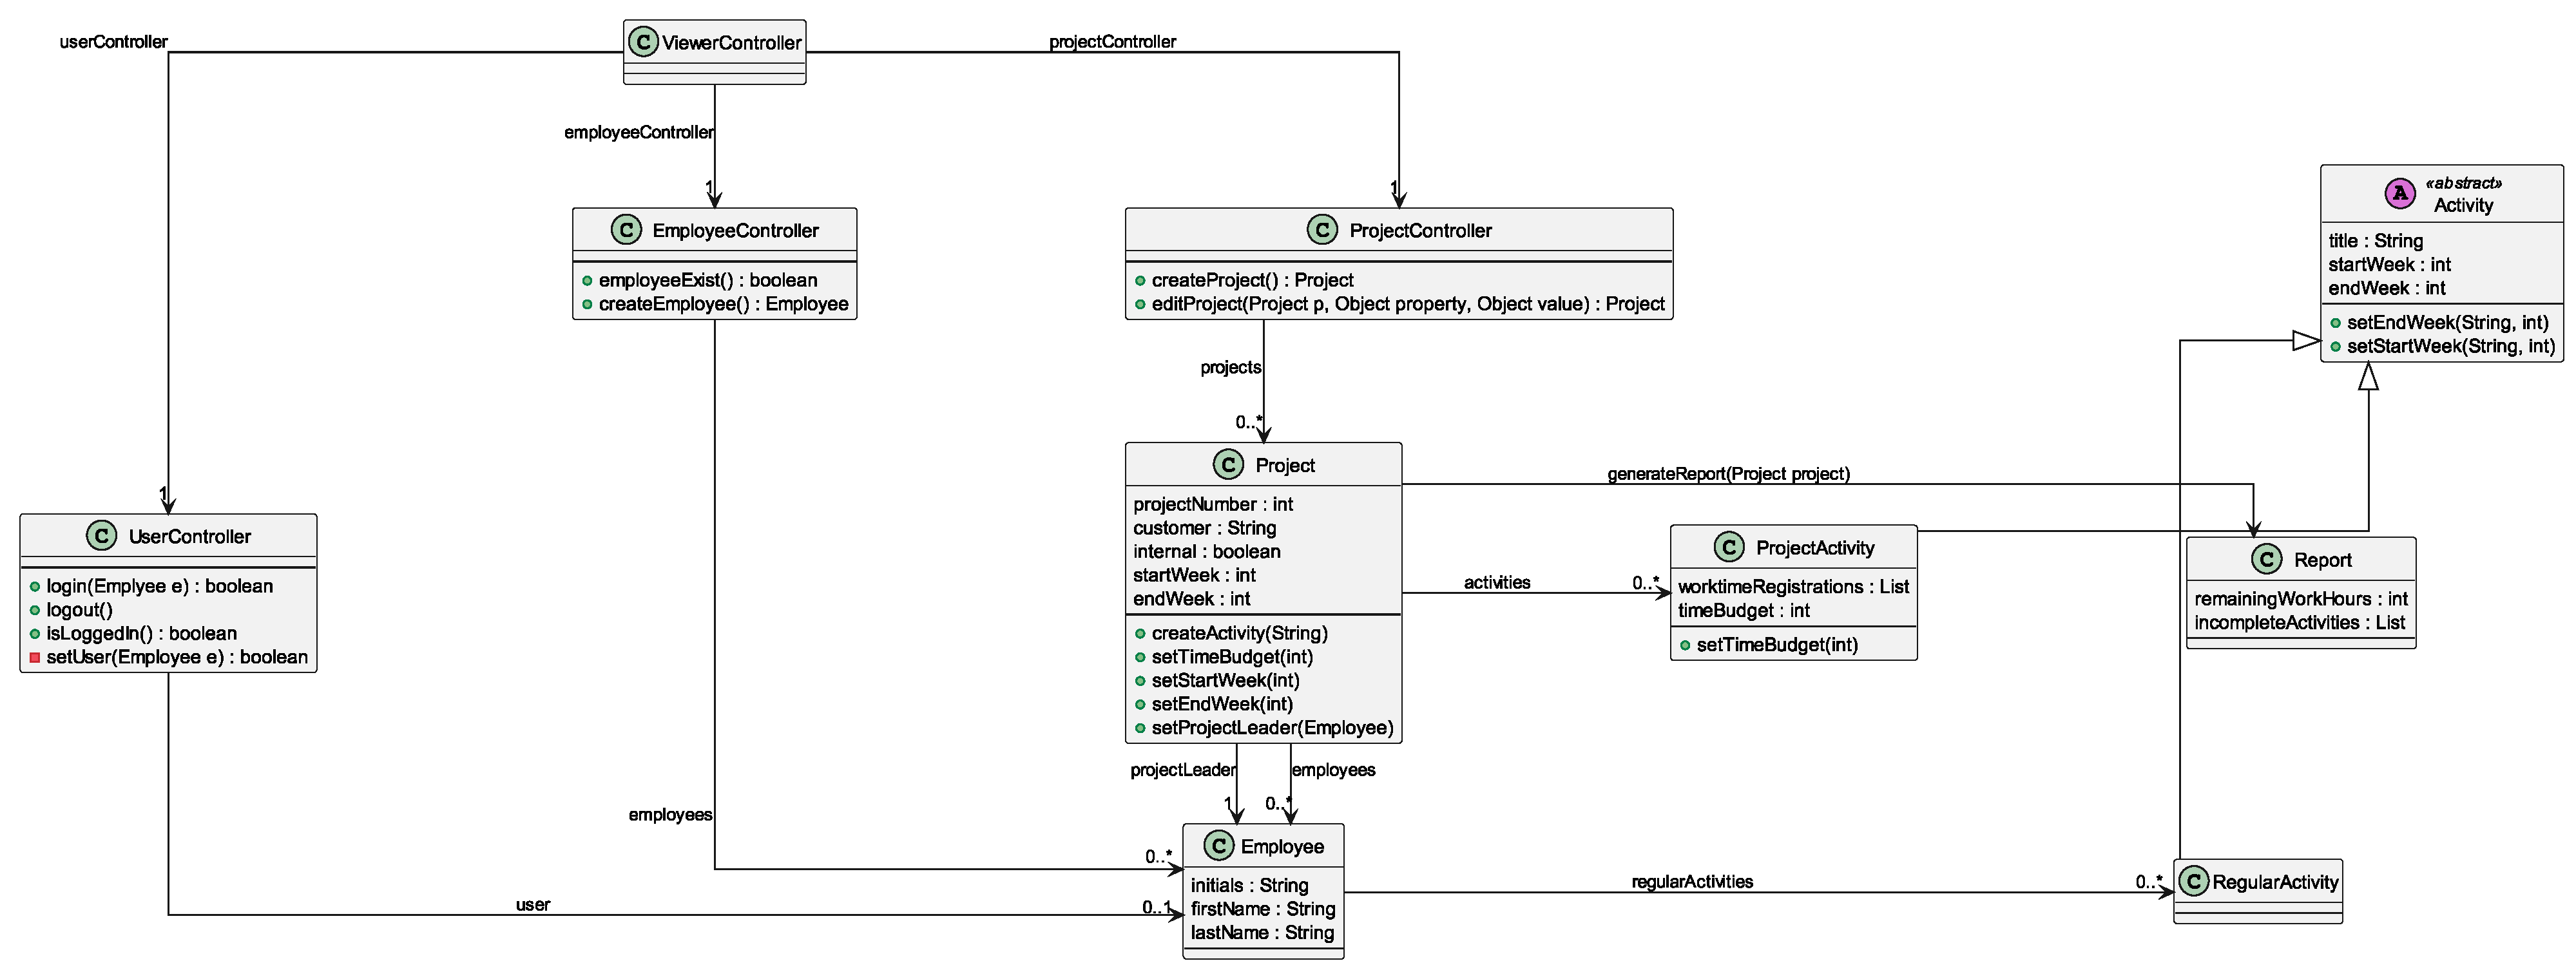
\includegraphics[width = \textwidth]{Diagrams/ClassDiagramMVC.eps}
\end{figure}
\subsection{Sekvensdiagrammer}\label{sec:sequence}
\begin{figure}[H]
    \centering
    \caption{Sekvensdiagram: Opret medarbejder}\label{fig:sequenceRegisterEmployee}
    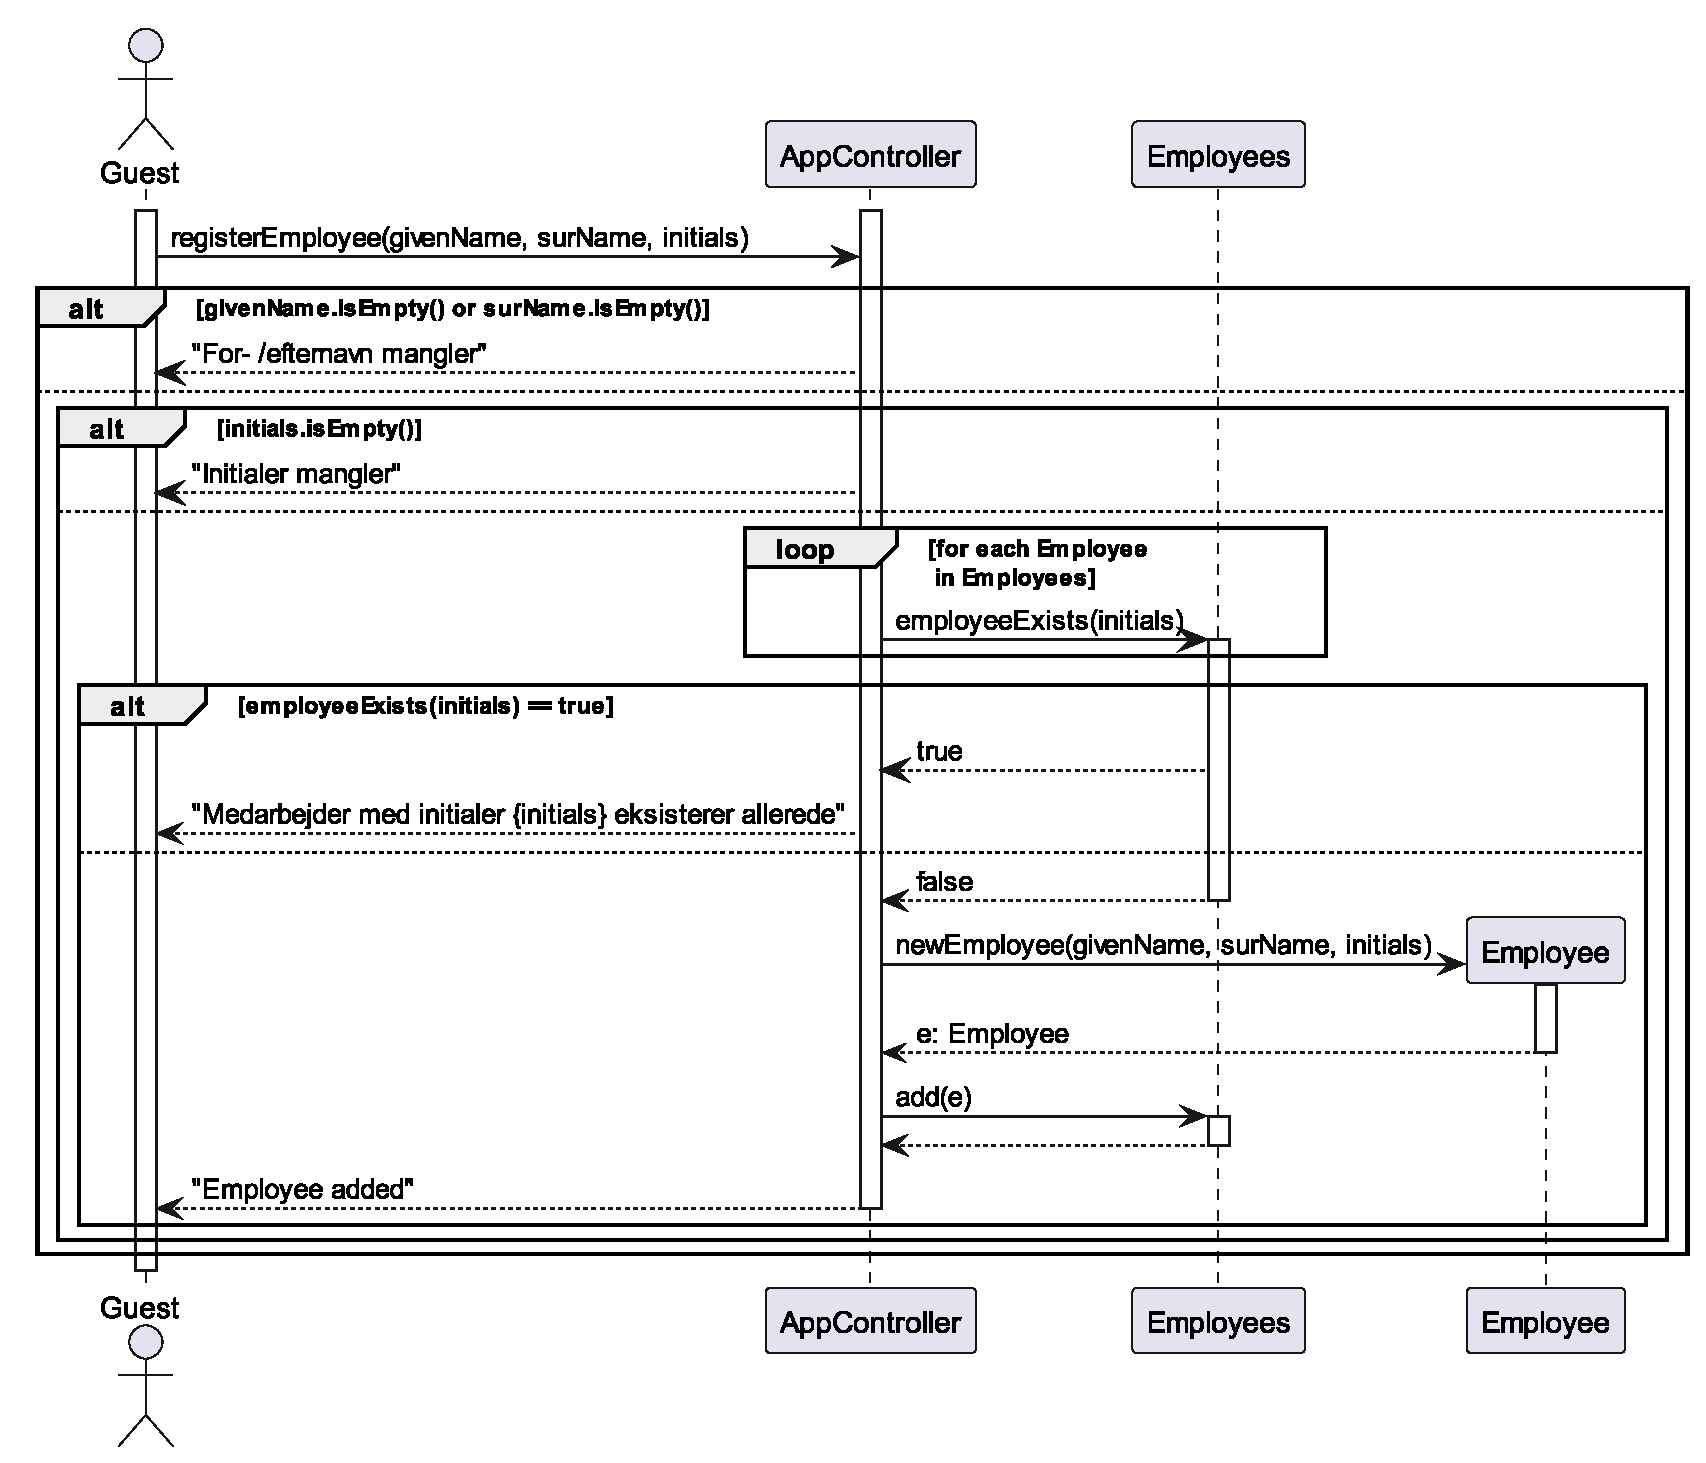
\includegraphics[width = .75\textwidth]{Diagrams/seq_registerEmployee.eps}
\end{figure}
\begin{figure}[H]
    \centering
    \caption{Sekvensdiagram: Medarbejder login}\label{fig:sequence_login}
    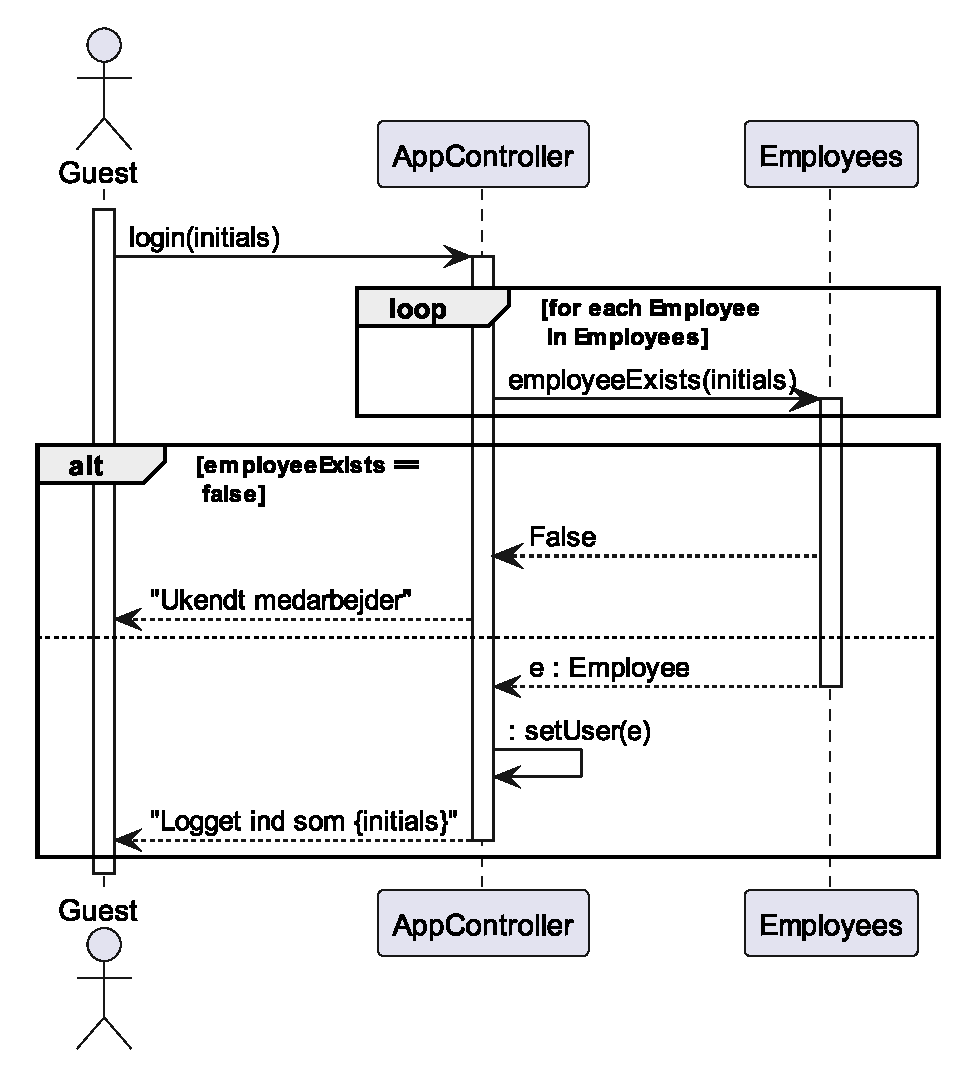
\includegraphics[width = .5\textwidth]{Diagrams/Login.eps}
\end{figure}
\begin{figure}[H]
    \centering
    \caption{Sekvensdiagram: Medarbejder log ud}\label{fig:sequence_logout}
    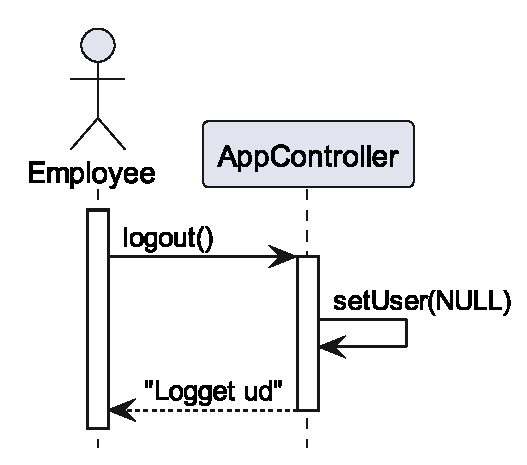
\includegraphics[width = .3\textwidth]{Diagrams/Logout.eps}
\end{figure}
\begin{figure}[H]
    \centering
    \caption{Sekvensdiagram: Opret projekt}\label{fig:sequence_create_project}
    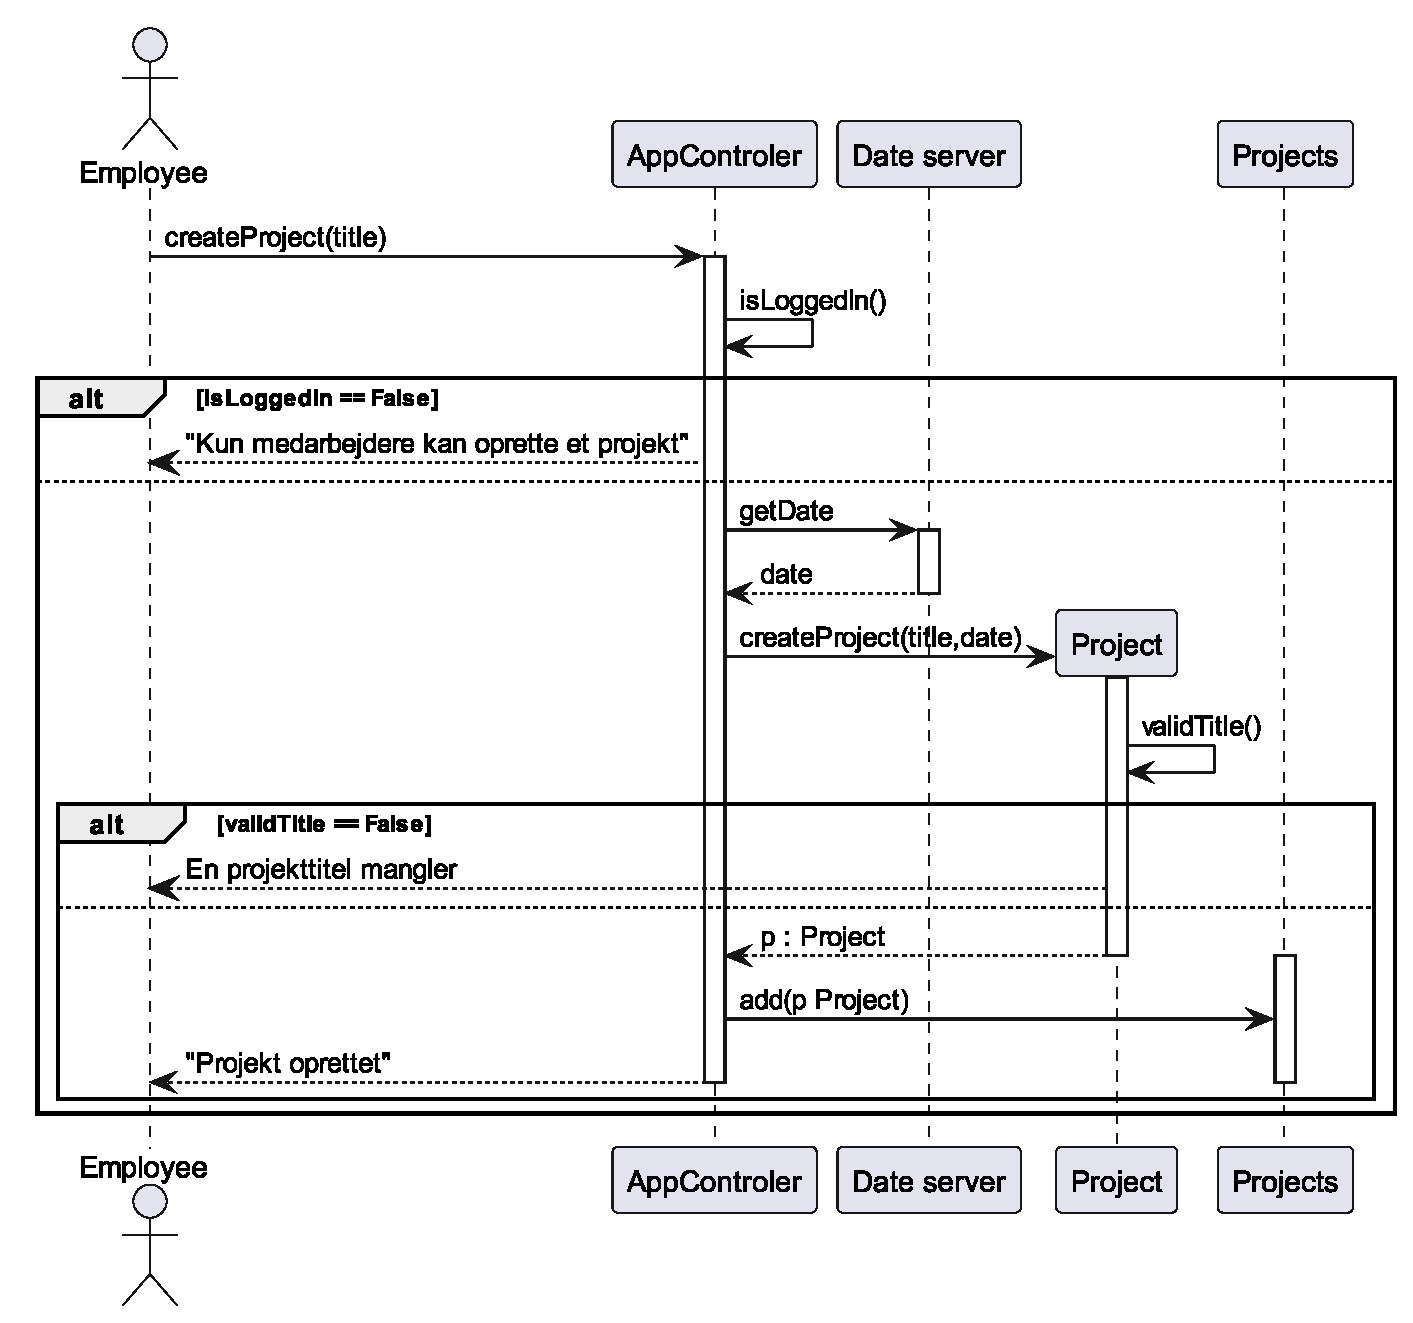
\includegraphics[width = .75\textwidth]{Diagrams/CreateProject.eps}
\end{figure}
\begin{figure}[H]
    \centering
    \caption{Sekvensdiagram: Forsøg på at oprette en projektaktivitet som gæst}\label{fig:sequence_create_PA_guest}
    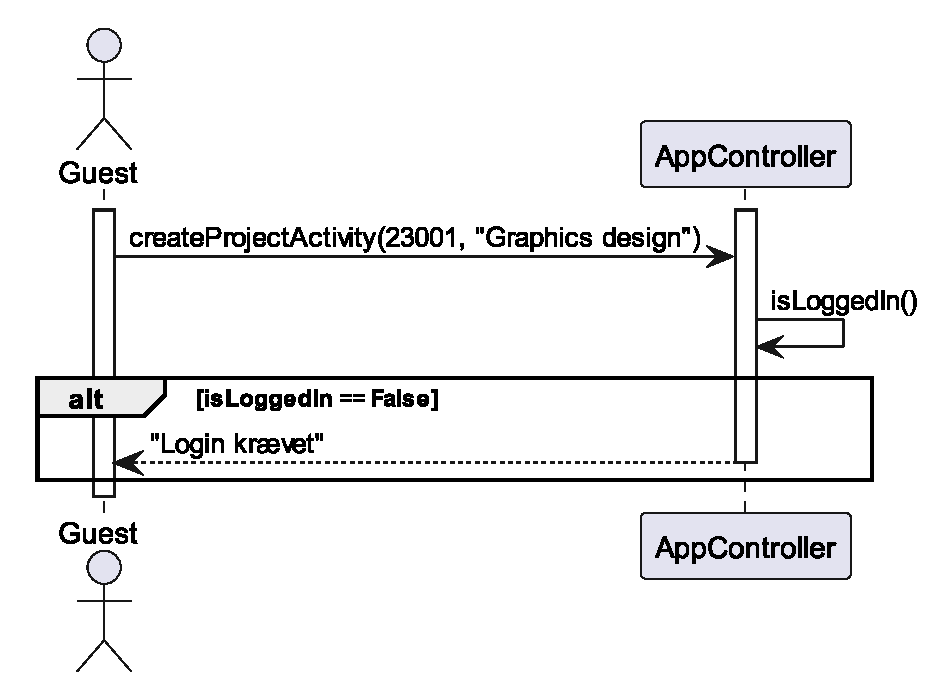
\includegraphics[width = .5\textwidth]{Diagrams/createActivityNoPLGuest.eps}
\end{figure}
\begin{figure}[H]
    \centering
    \caption{Sekvensdiagram: Forsøg på at oprette en projektaktivitet på projekt uden projektleder}\label{fig:sequence_create_PA_no_PL_1}
    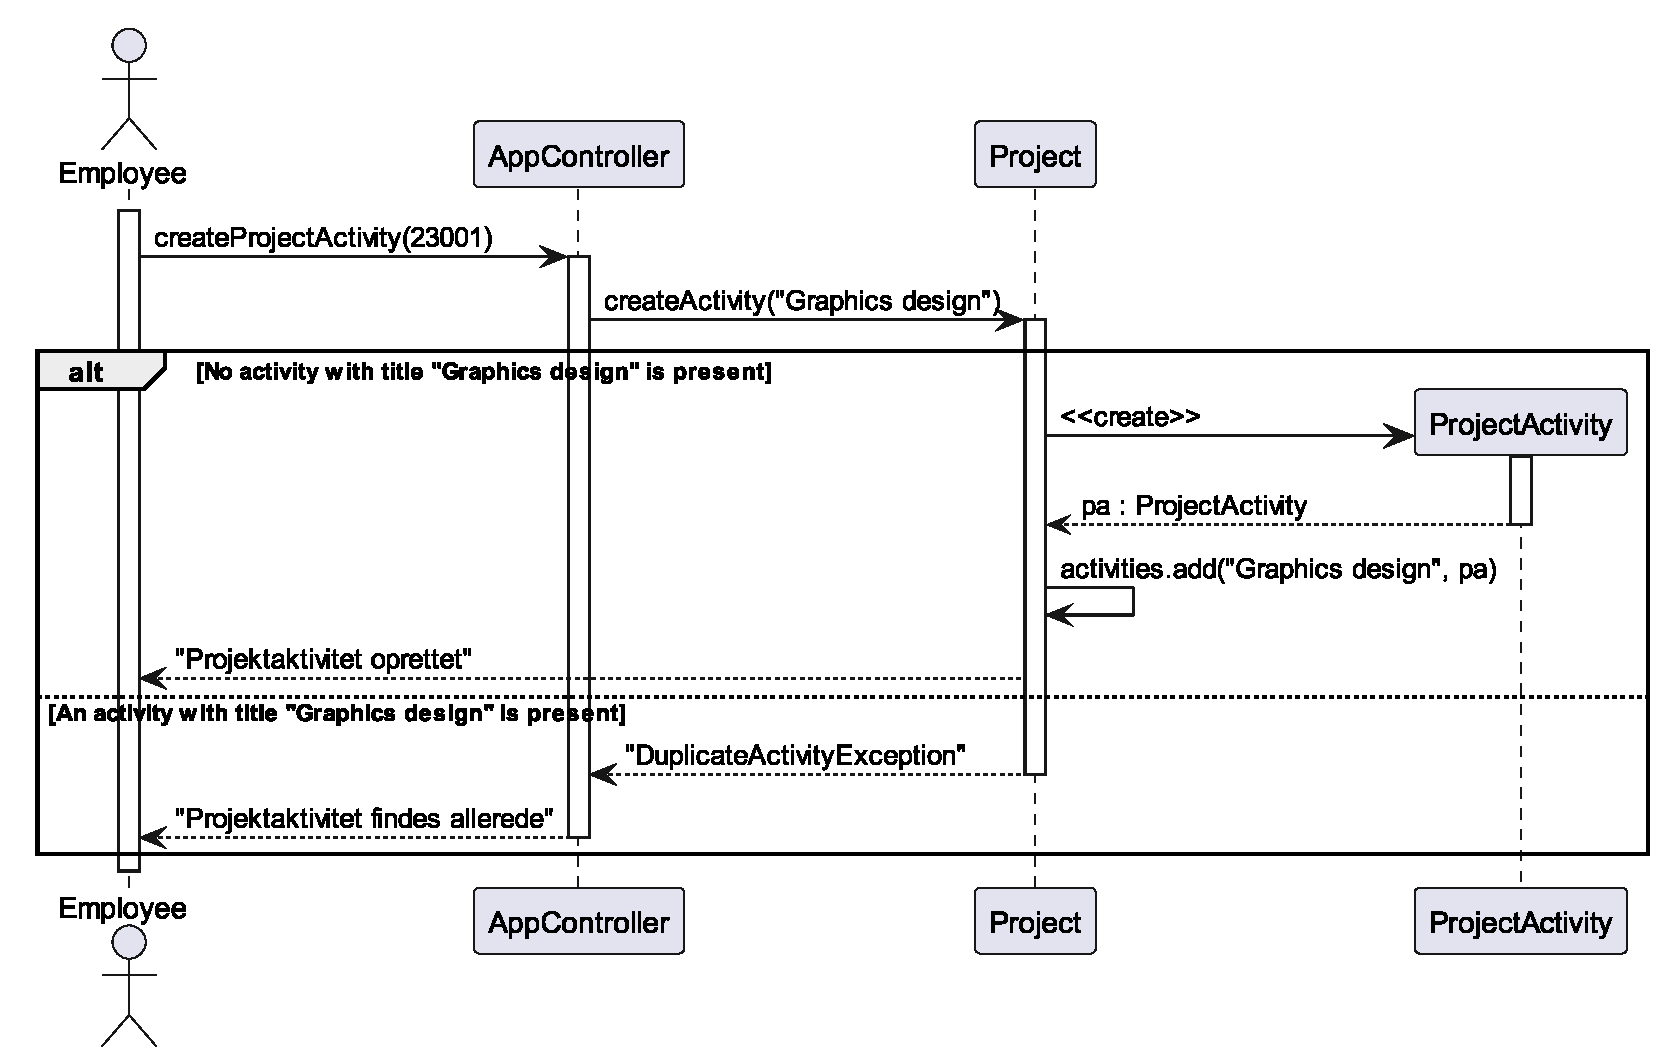
\includegraphics[width = .75\textwidth]{Diagrams/createActivityNoPLCase1.eps}
\end{figure}
\begin{figure}[H]
    \centering
    \caption{Sekvensdiagram: Forsøg på at fastsætte timebudget på projekt uden projektleder}\label{fig:sequence_create_PA_no_PL_2}
    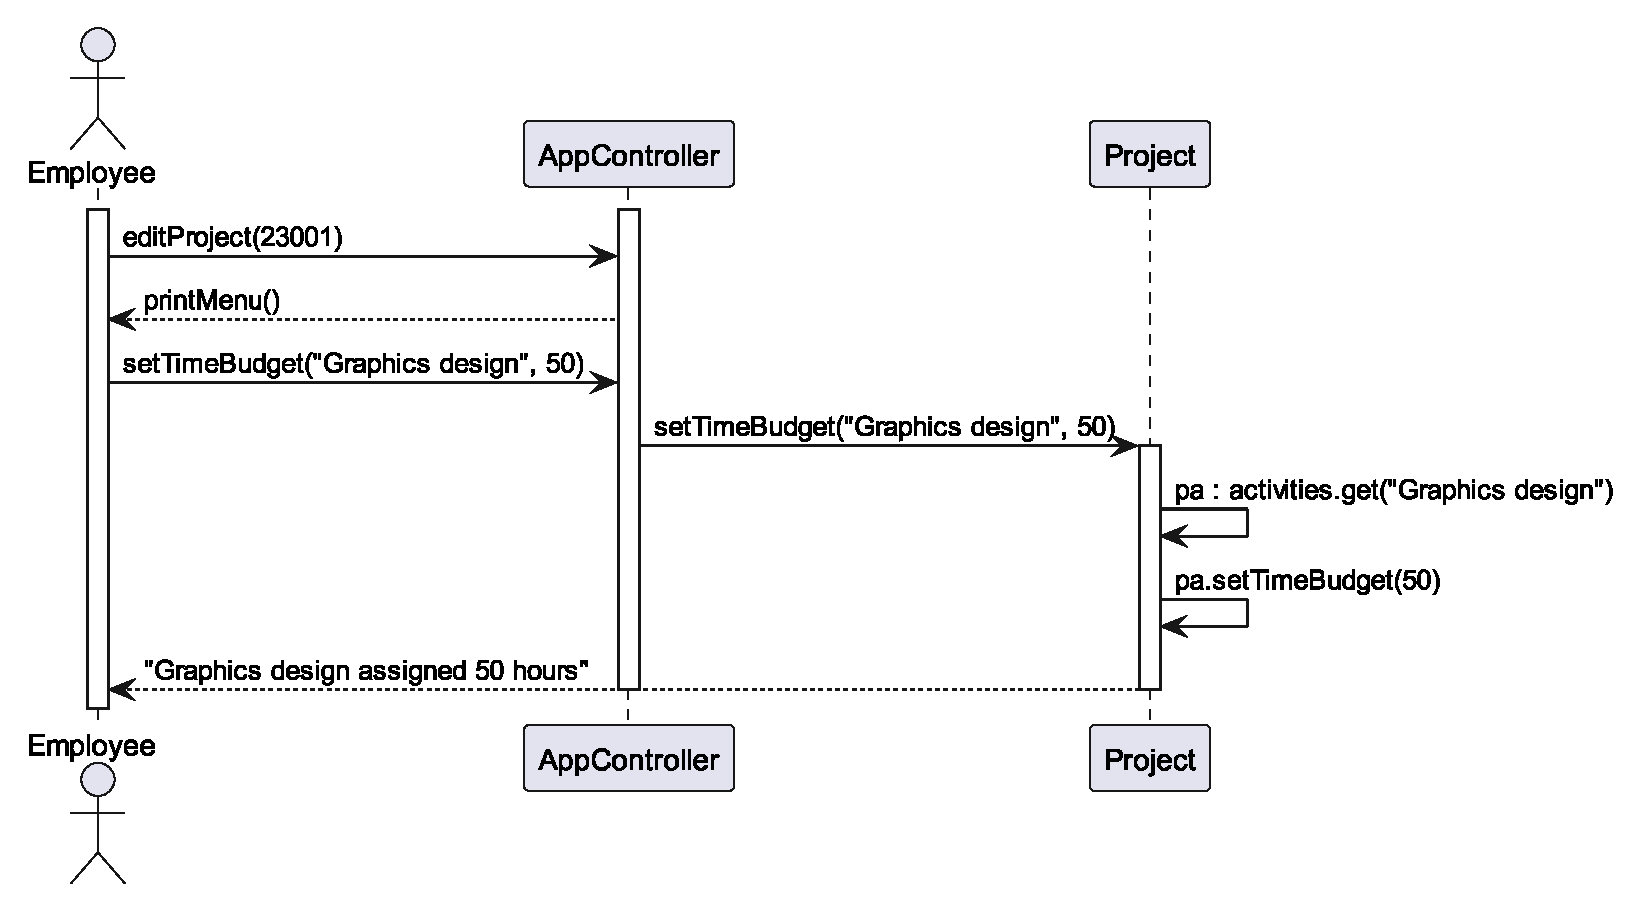
\includegraphics[width = .75\textwidth]{Diagrams/createActivityNoPLCase2.eps}
\end{figure}
\begin{figure}[H]
    \centering
    \caption{Sekvensdiagram: Forsøg på at fastsætte startuge på projekt uden projektleder}\label{fig:sequence_create_PA_no_PL_3}
    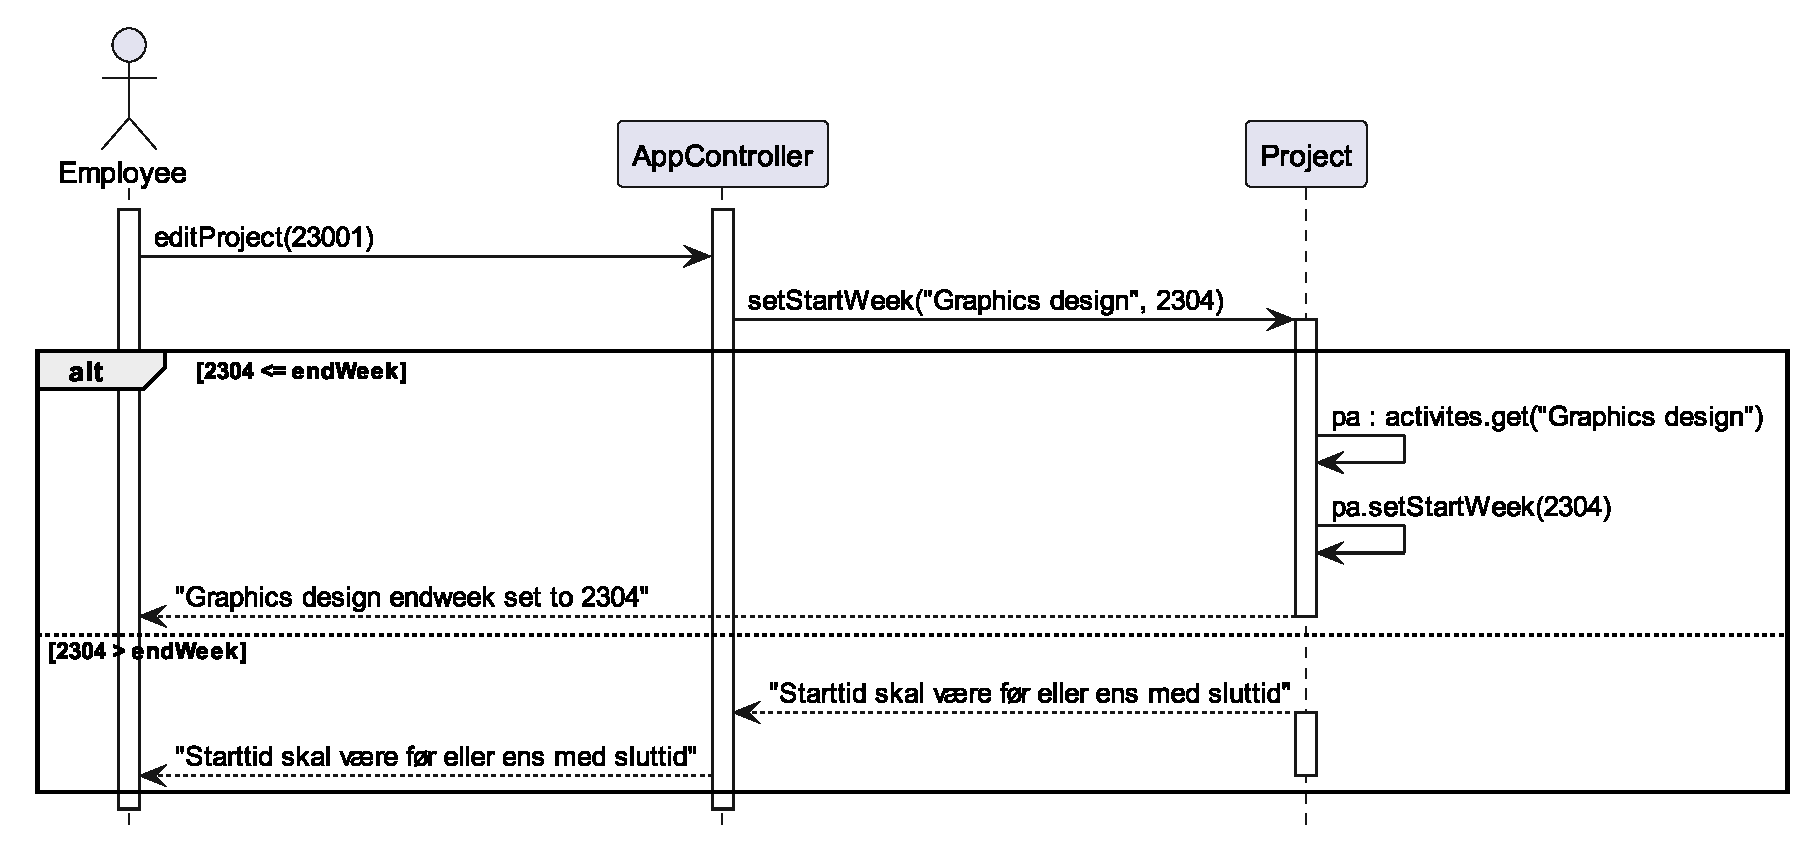
\includegraphics[width = .9\textwidth]{Diagrams/createActivityNoPLCase3.eps}
\end{figure}
\begin{figure}[H]
    \centering
    \caption{Sekvensdiagram: Forsøg på at fastsætte slutuge på projekt uden projektleder}\label{fig:sequence_create_PA_no_PL_4}
    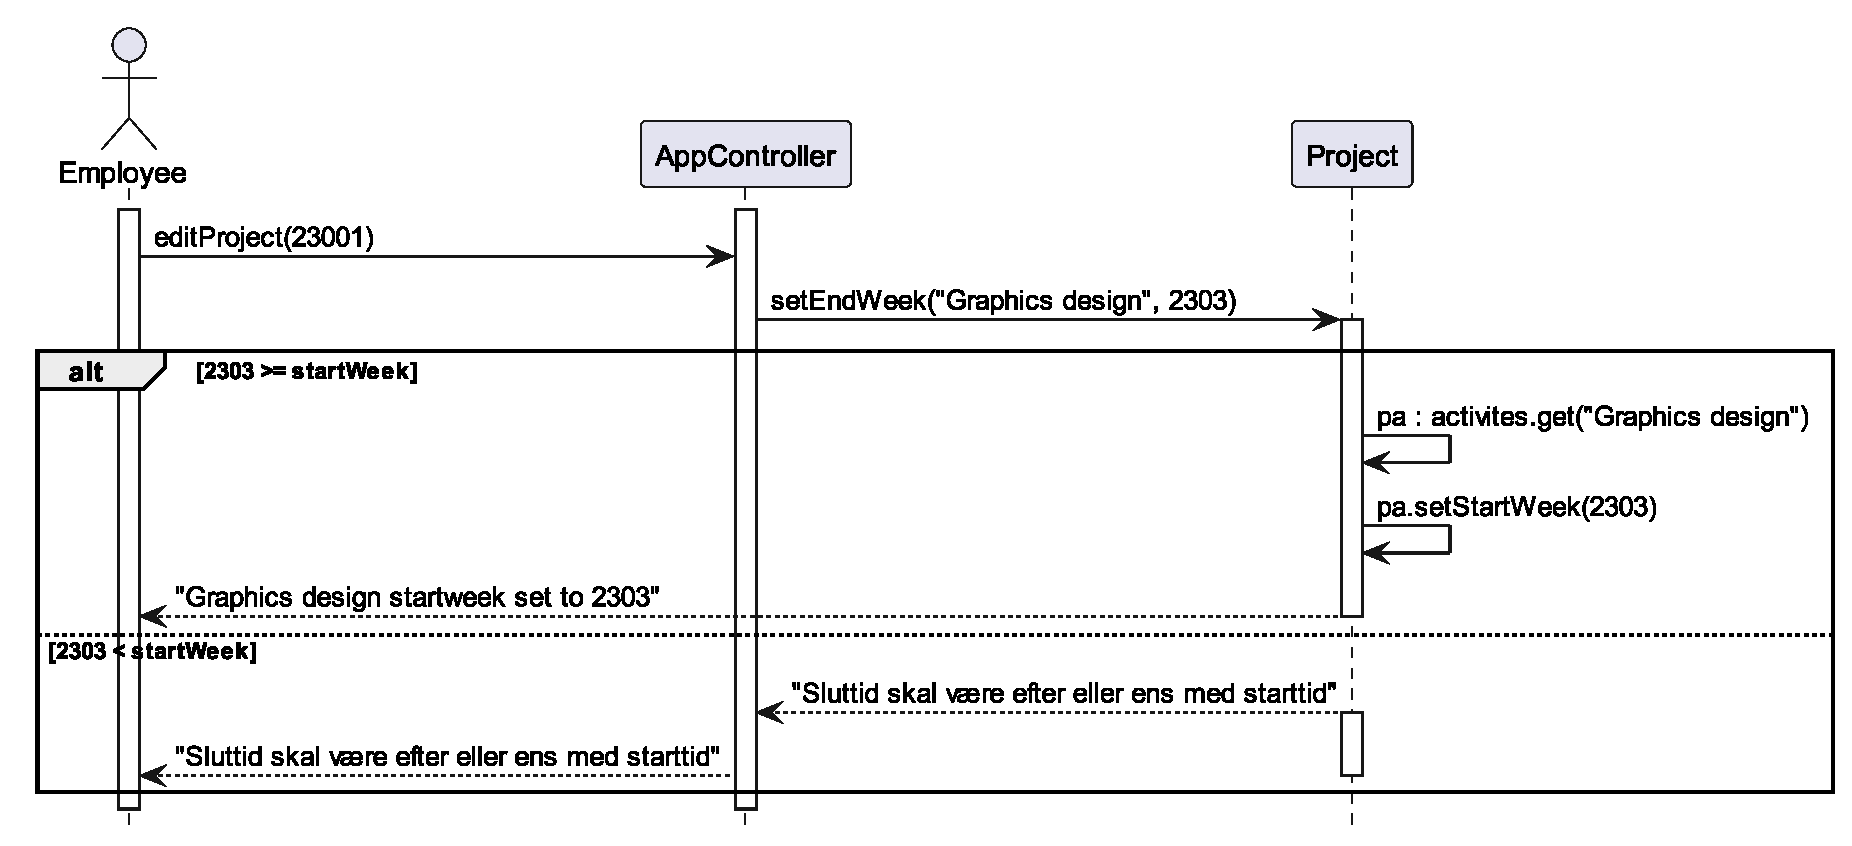
\includegraphics[width = .9\textwidth]{Diagrams/createActivityNoPLCase4.eps}
\end{figure}
\begin{figure}[H]
    \centering
    \caption{Sekvensdiagram: Forsøg på at oprette en projektaktivitet på et projekt med en projektleder}\label{fig:sequence_create_PA_PL}
    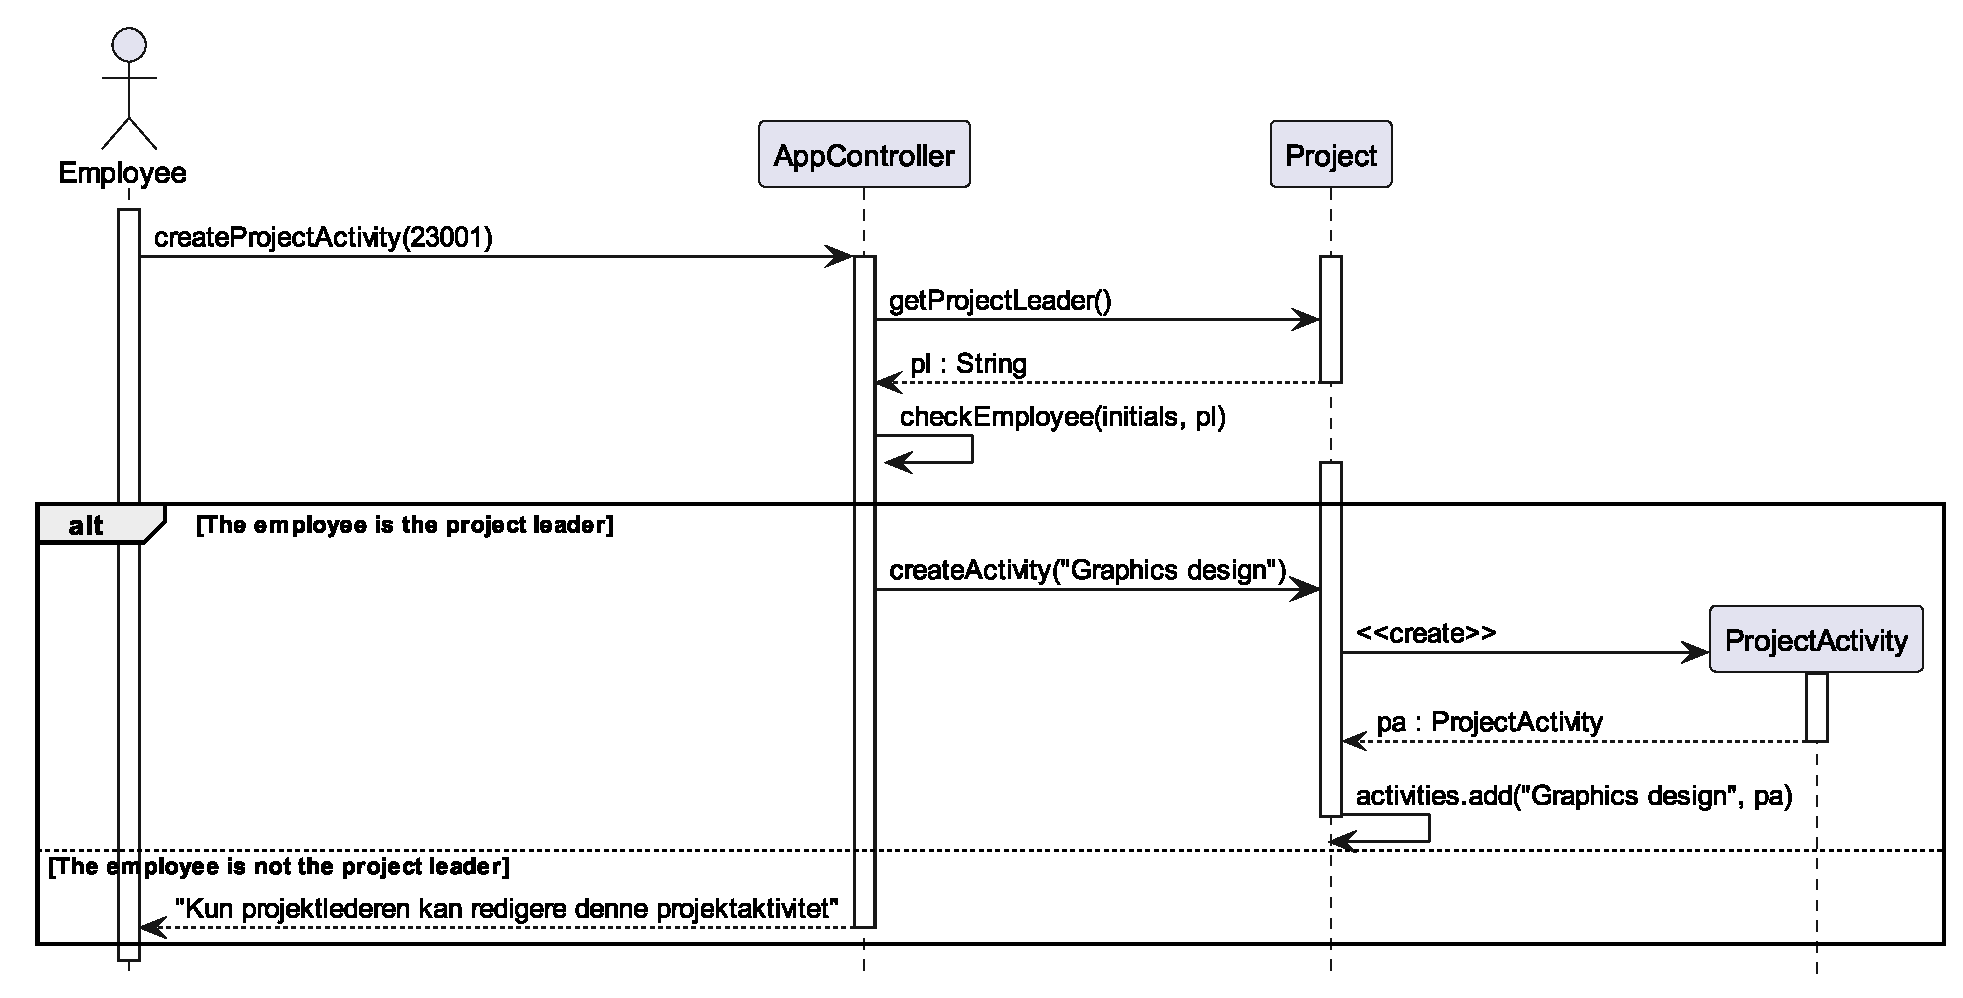
\includegraphics[width = .95\textwidth]{Diagrams/createActivityPL.eps}
\end{figure}
\begin{figure}[H]
    \centering
    \caption{Sekvensdiagram: Rediger projekt}\label{fig:sequence_project_edit}
    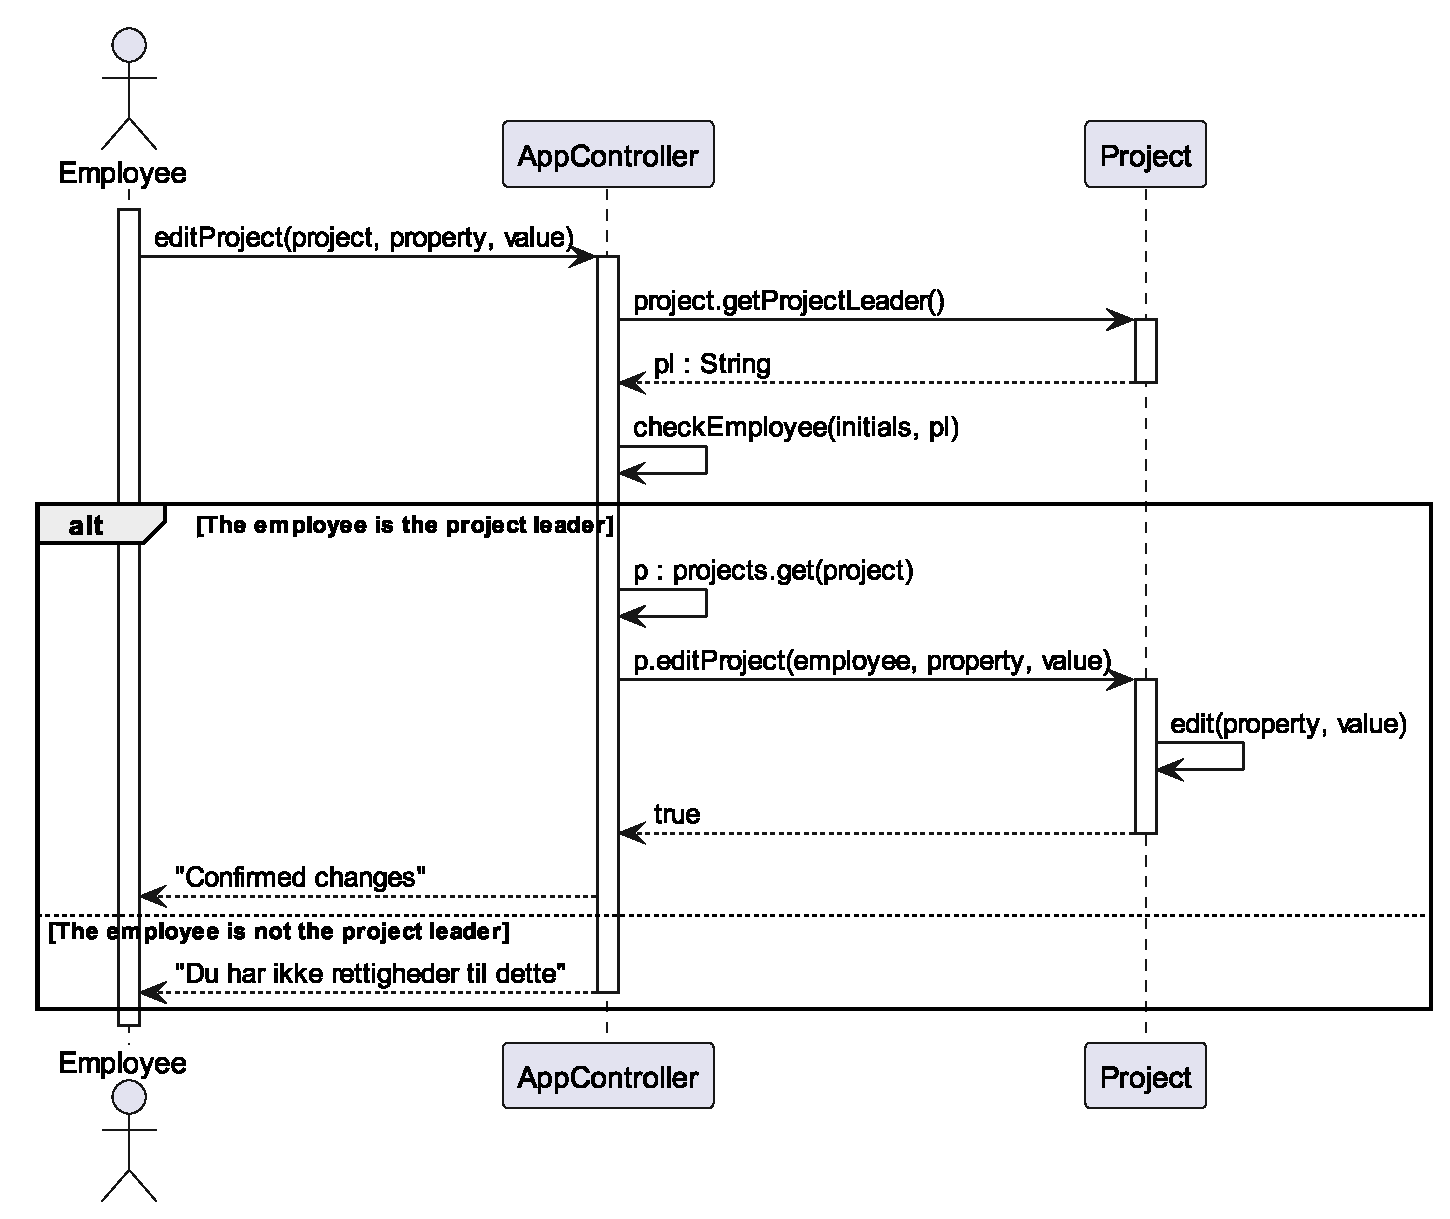
\includegraphics[width = .75\textwidth]{Diagrams/seq_project_edit.eps}
\end{figure}
\begin{figure}[H]
    \centering
    \caption{Sekvensdiagram: Medarbejder udpeger sig som projektleder}\label{fig:becomeProjectLeader}
    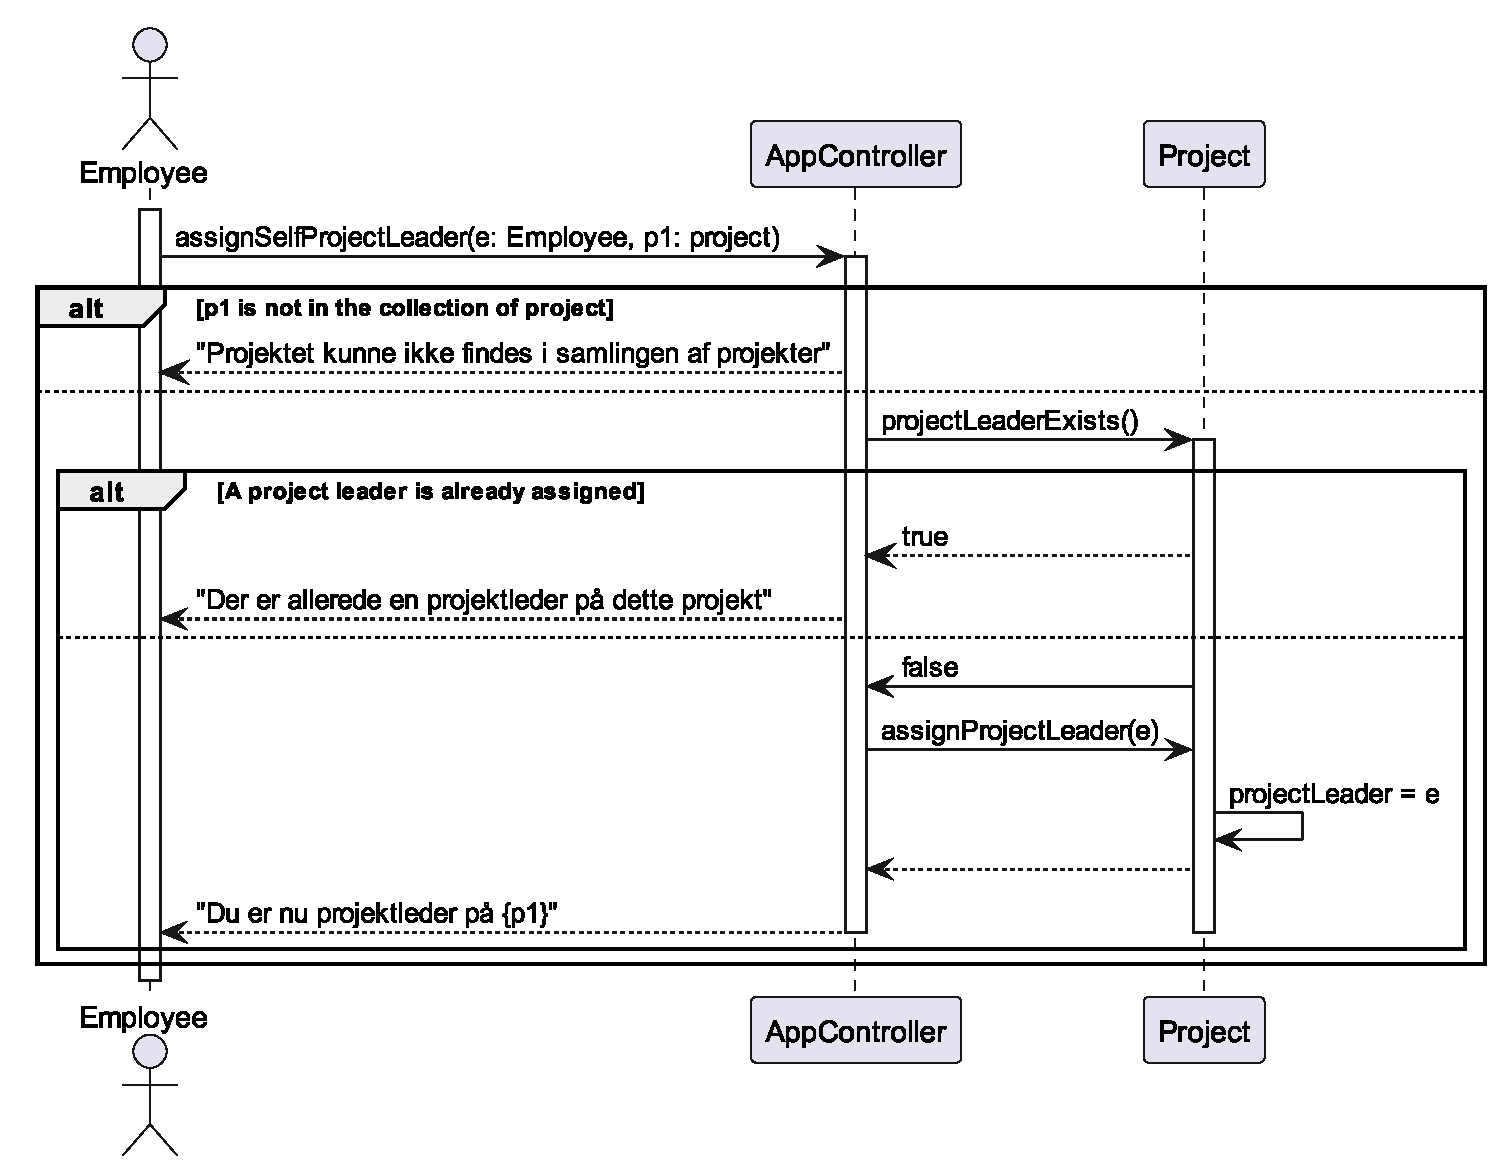
\includegraphics[width = 1\textwidth]{Diagrams/BecomeProjectLeader.eps}
\end{figure}
\newpage
\section{Diskussion: Programdesign}
I dette afsnit bearbejdes to ting kort:
\begin{enumerate}
    \item Valg af datastrukturer
    \item Valg af klassestrukturer
\end{enumerate}
\subsection{Datastrukturer} I valg af datastrukturer er det vigtigt hvorledes vi henter og gemmer data. I programmet bliver medarbejdere og aktiviteter defineret med en unik streng, mens projekter bliver defineret med et løbenummer. Hvis man for nemheds skyld konverterer løbenummeret til en streng, er der mulighed for at alle tre objekter kan gemmes i Map strukturer. Dette gør det nemt at hente objekter med \mintinline{java}|.get(key)|, udføre operationer på objekterne og overskrive objekterne i Map'et med \mintinline{java}|.put(key, Object)|. Er det nødvendigt at iterere over et Map, kan man også nemt bruge Java's \mintinline{java}|.stream()| metode. Ønsker man at gemme brugt arbejdstid på en aktivitet er det derimod nemmest at gemme denne i en List, da arbejdstiden kun akkumuleres.
\subsection{Klassestrukturer} Programmet skal holdes simpelt og objekter skal nødvendigvis eje hinanden på en simpel måde. Det er besluttet at en \emph{Controller/Model}-klasse varetager programmets busniessstruktur. Hvis klassen bliver for kompliceret kan der senere indsættes en \emph{Viewer/Controller}-klasse som udelukkende varetager UI. Controller klassen indeholder Maps med projekter, medarbejdere og rapporter. Aktiviteter eksistere som en abstrakt klasse der nedarves til en fast aktivitet (f.eks. ferie), og projekt aktiviteter. De faster kan så ejes af et medarbejder objekt. Projektaktiviteter ejes af projekt objekter. Dermed bliver aktivitetsobjekter så ens som muligt, men ejes af de objekter der skal bruge dem. Med valget af MVC (Model-View-Controller)-arkitektur er der fare for at man som udvikler kan gøre controller-objekter til "gudeklasser", dog egner denne abstraktion sig særligt godt til planlægningsarbejdet, da man ved opmærksomhed på denne fare tvinges til at betragte cohesion og coupling endnu nærmere, end man måske ville have gjort uden den. Ligeledes deler den data og handlinger på de data naturligt (og ansvar), hvilket er en central idé i objektorienteret programmering. Endeligt er det et arkitekturmønster der naturligt passer på denne opgave jf. Softwarehuset's requirements; modellen er i vores tilfælde objekter der repræsenterer projektdata, viewet er vores brugergrænseflade og lader bl.a. Softwarehuset skabe overblik gennem rapporter, og kan vise hvilke medarbejdere er ledige til et projekt. Controlleren udbyder muligheden for at ændre objekterne (f.eks. til registrere arbejdstid, registrere ferie/sygdom og modifikation af projekter).